\documentclass[aspectratio=169,11pt,xcolor=dvipsnames]{beamer}
\usepackage{graphicx} % For including graphics.
\usepackage{hyperref} % For links.
\usepackage{multirow}
\usepackage{minted}

\title{Computer Graphics with Clojure, LWJGL, and Fastmath}
\author{Jan Wedekind}
\date{Saturday, October 18th 2025}

\hypersetup{pdftitle          = {Computer Graphics with Clojure, LWJGL, and Fastmath},
            pdfsubject        = {rendering NASA CGI Moon Kit data using Clojure, LWJGL, and Fastmath},
            pdfauthor         = {Jan Wedekind},
            pdfkeywords       = {Clojure, LWJGL, Fastmath, rendering, NASA, Moon, graphics},
            pdfcreator        = {LaTeX with Beamer class},
            pdfproducer       = {TeX Live 2025/dev/Debian},
            bookmarksopen     = false,
            bookmarksnumbered = true,
            colorlinks        = true,
            filecolor         = cyan,
            citecolor         = green,
            linkcolor         = blue,
            urlcolor          = blue}

\usebackgroundtemplate{
\includegraphics[width=\paperwidth,height=\paperheight]{slide}}

\setbeamersize{text margin left=0.25cm,
               text margin right=0.25cm}

\usecolortheme{seahorse}



\definecolor{slidecolor}{rgb}{0.65,0.71,0.72}
\setbeamercolor{titlelike}{fg=black,bg=slidecolor!60}
\setbeamercolor{frametitle}{fg=black,bg=slidecolor!100}

\begin{document}

\begin{frame}
  \pdfbookmark[1]{Computer Graphics with Clojure, LWJGL, and Fastmath}{title}
  \titlepage{}
\end{frame}

\begin{frame}
  \pdfbookmark[1]{About Me}{bio}
  \frametitle{About Me}
  \begin{minipage}[b]{0.79\textwidth}
    \begin{itemize}
      \item As a kid: playing with Omikron Basic, Borland Pascal
      \item Computer Science at Karlsruhe University
        \begin{itemize}
          \item compiler construction, robotics, measurement engineering
        \end{itemize}
      \item PhD on Computer Vision using Ruby at Sheffield Hallam University
      \item Computer Vision and Machine Learning in Industry
        \begin{itemize}
          \item Using C++, Ruby, Python
        \end{itemize}
      \item Hobby projects
        \begin{itemize}
          \item C++, Ruby, GNU Guile, Clojure
        \end{itemize}
    \end{itemize}
  \end{minipage}
  \begin{minipage}[b]{0.2\textwidth}
    
\includegraphics[width=\textwidth]{avatar}\\
    \begin{tiny}
      \url{https://www.wedesoft.de/}
    \end{tiny}
  \end{minipage}
\end{frame}

\begin{frame}
  \pdfbookmark[1]{Space Flight Simulator Examples}{stateoftheart}
  \frametitle{Space Flight Simulator Examples}
  \begin{minipage}[t]{0.49\textwidth}
    \begin{center}
      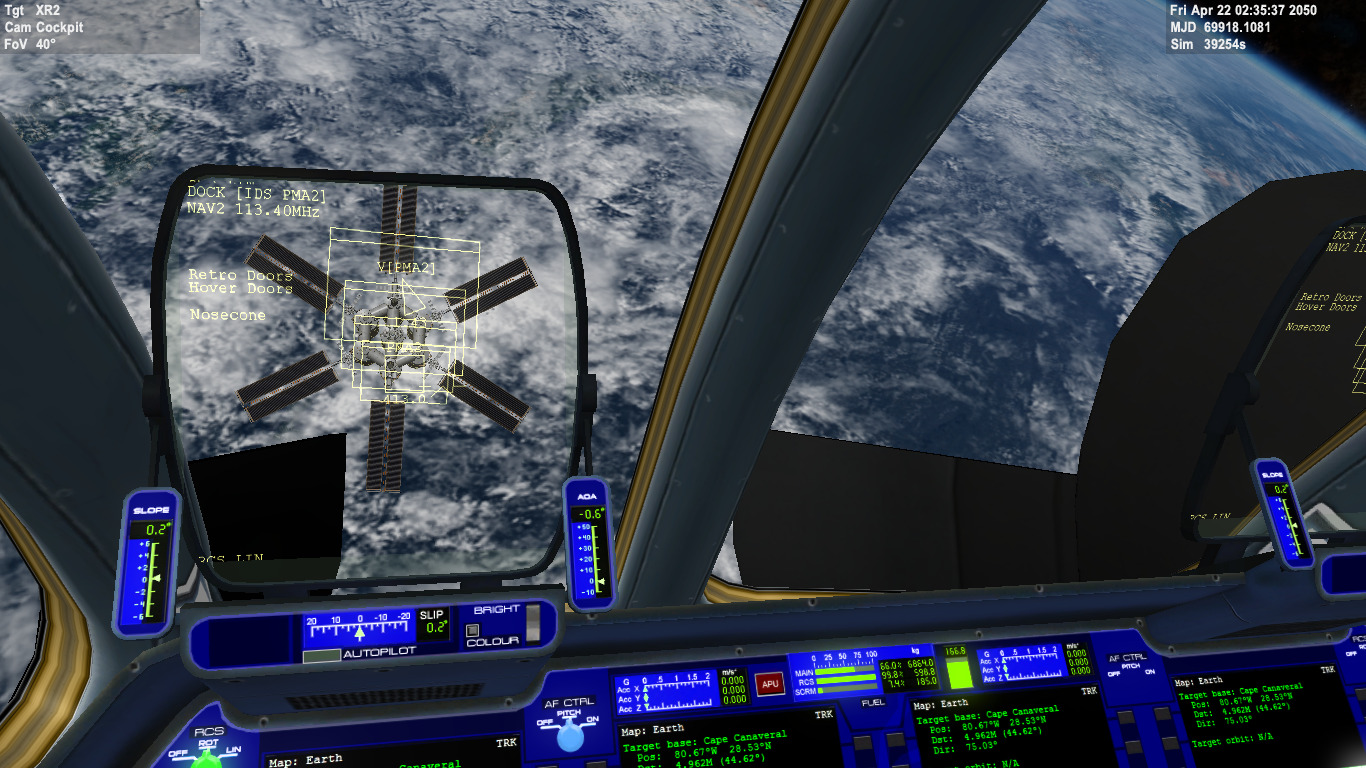
\includegraphics[width=\textwidth]{orbiter}\\
      \href{https://openorbiter.space/}{Open Orbiter Sim}
    \end{center}
  \end{minipage}
  \begin{minipage}[t]{0.49\textwidth}
    \begin{center}
      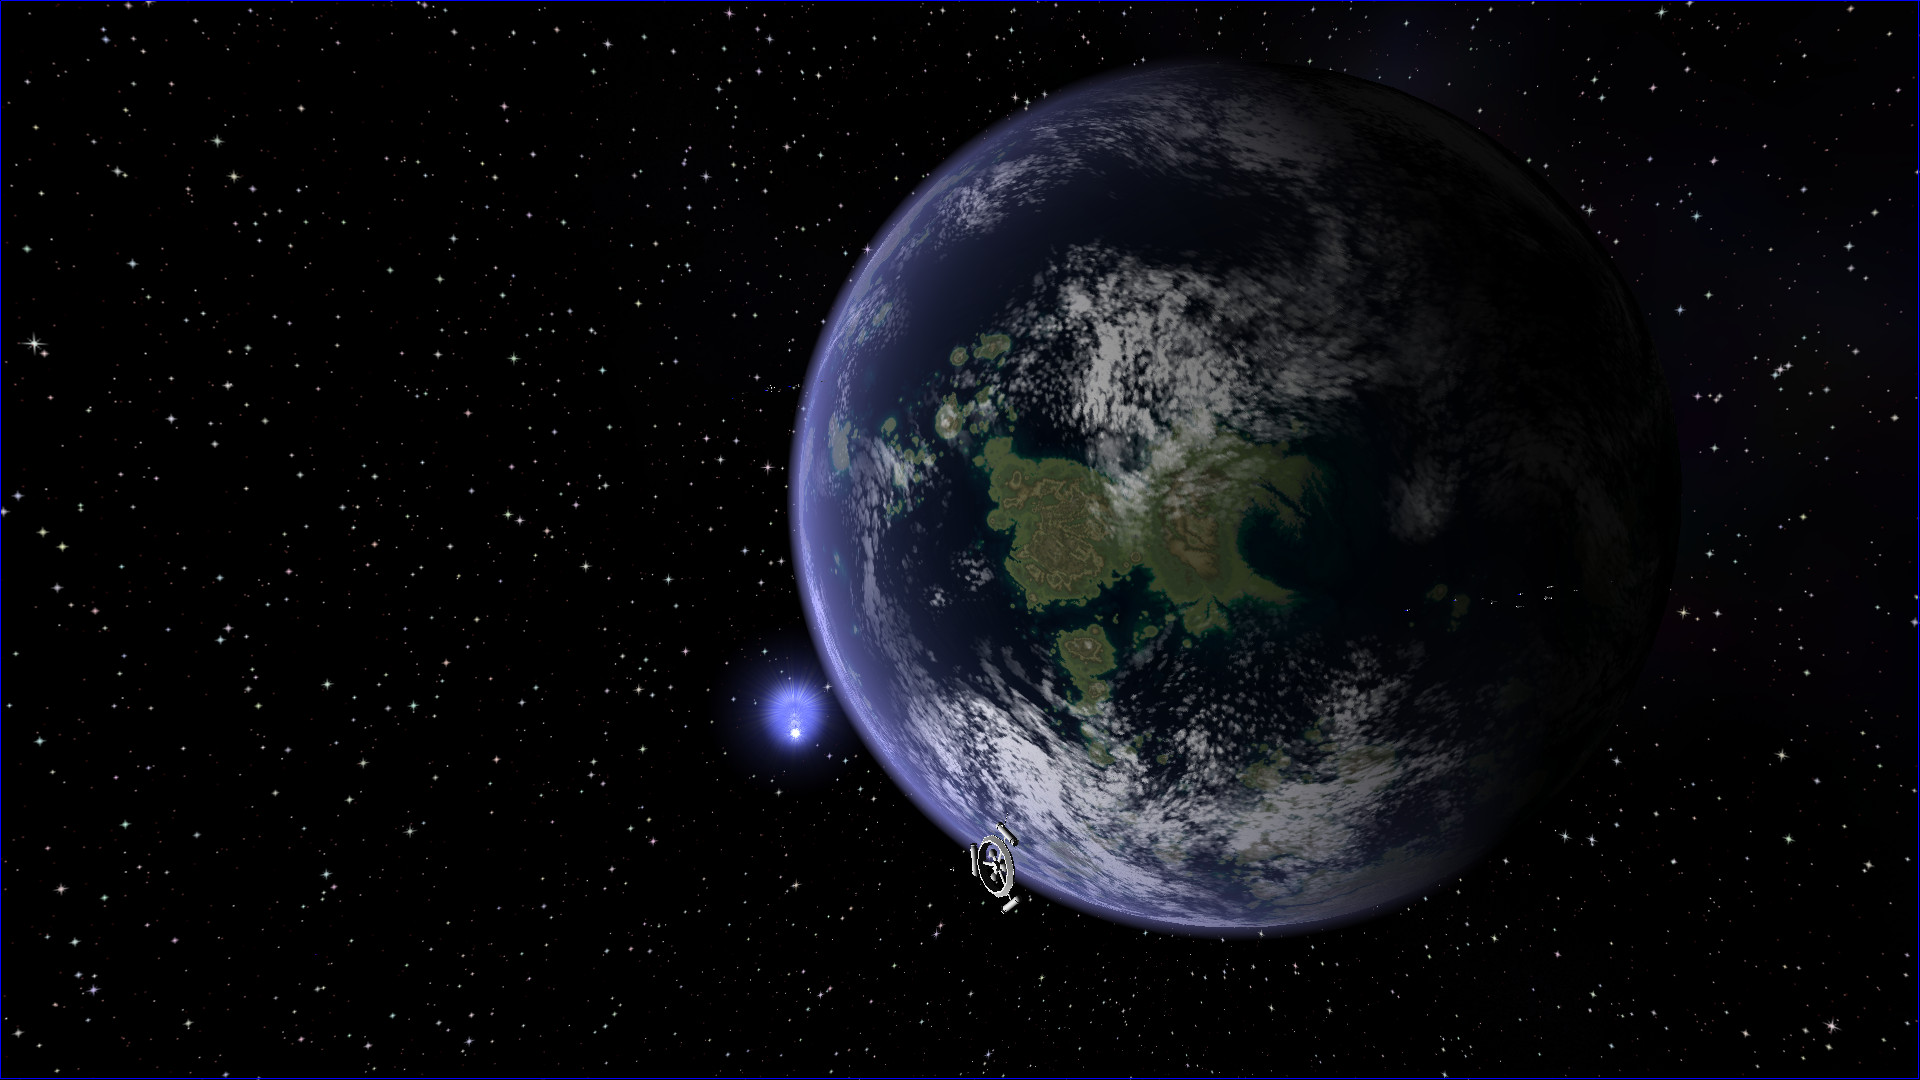
\includegraphics[width=\textwidth]{nerds}\\
      \href{https://smcameron.github.io/space-nerds-in-space/}{Space Nerds in Space}
    \end{center}
  \end{minipage}
\end{frame}

\begin{frame}
  \frametitle{Space Flight Simulator Examples}
  \begin{minipage}[t]{0.49\textwidth}
    \begin{center}
      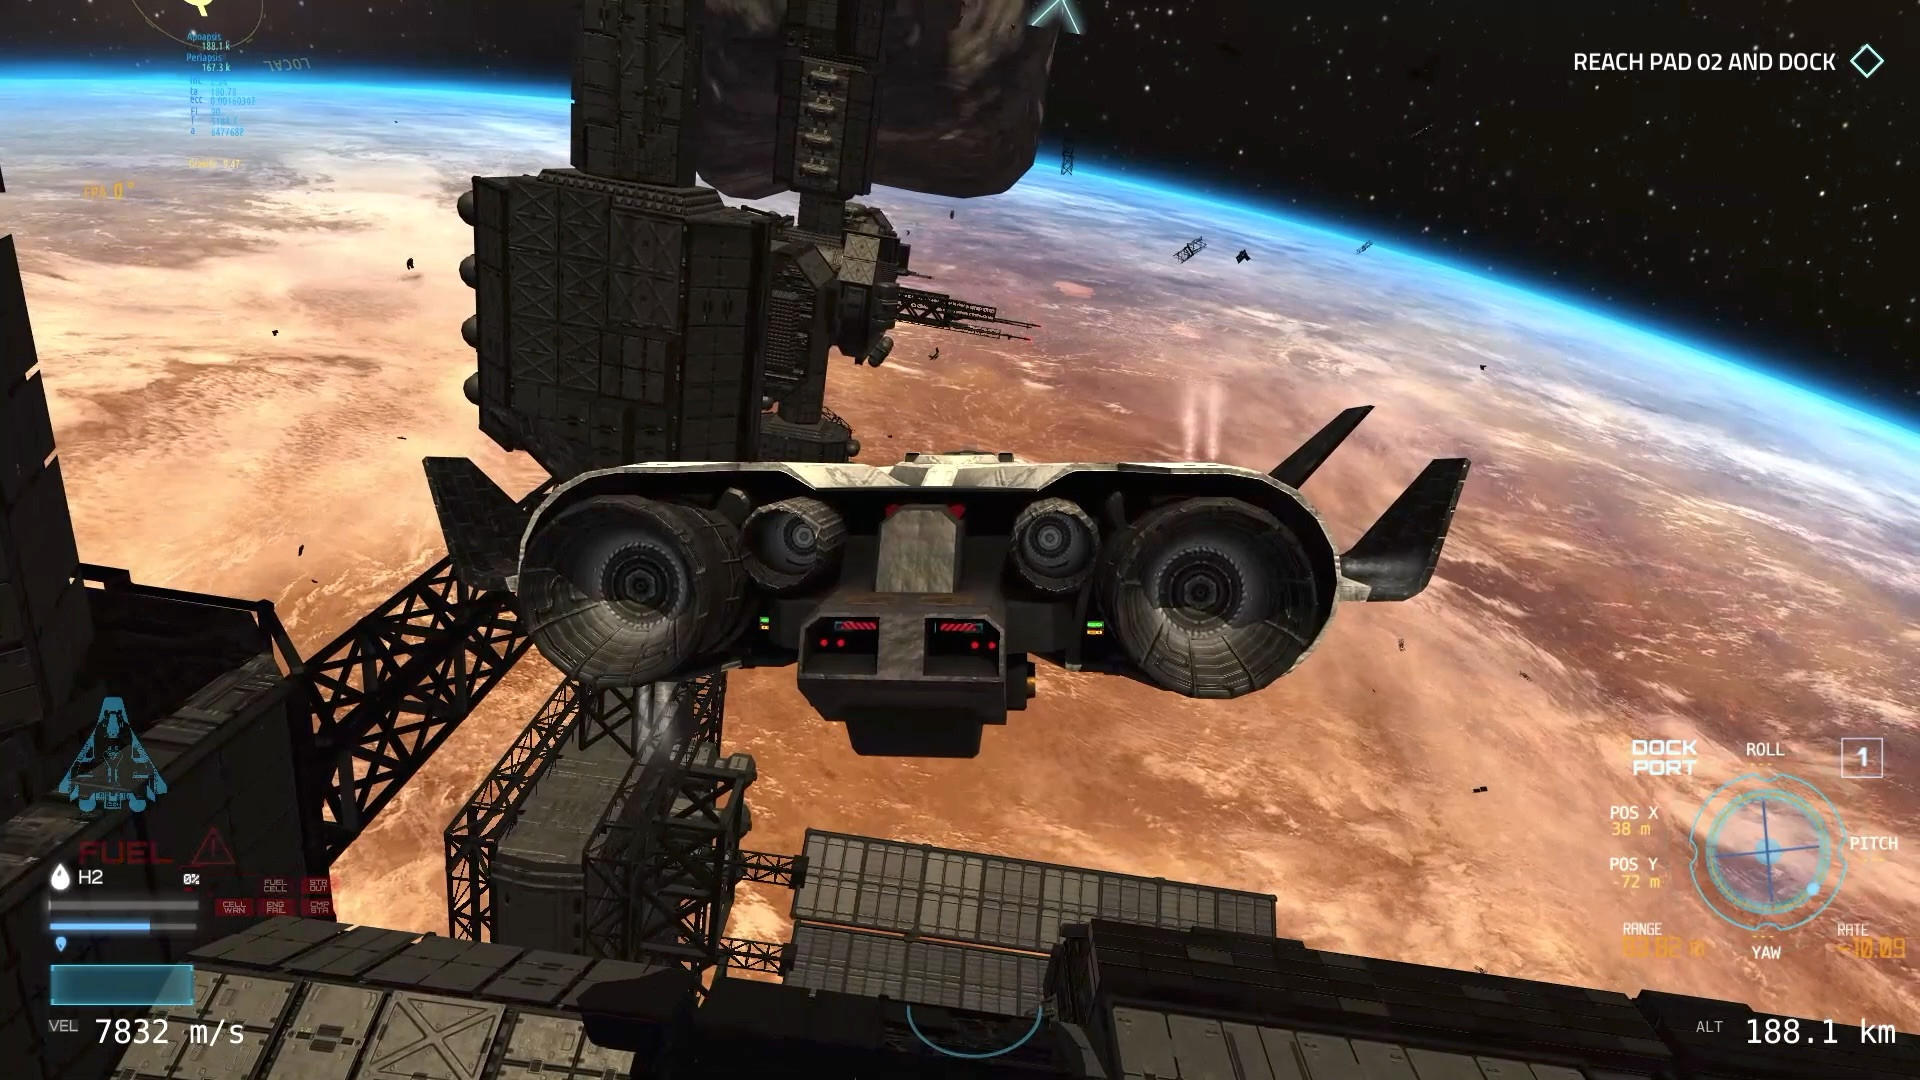
\includegraphics[width=\textwidth]{flight-of-nova}\\
      \href{https://flight-of-nova.com/}{Flight of Nova}
    \end{center}
  \end{minipage}
  \begin{minipage}[t]{0.49\textwidth}
    \begin{center}
      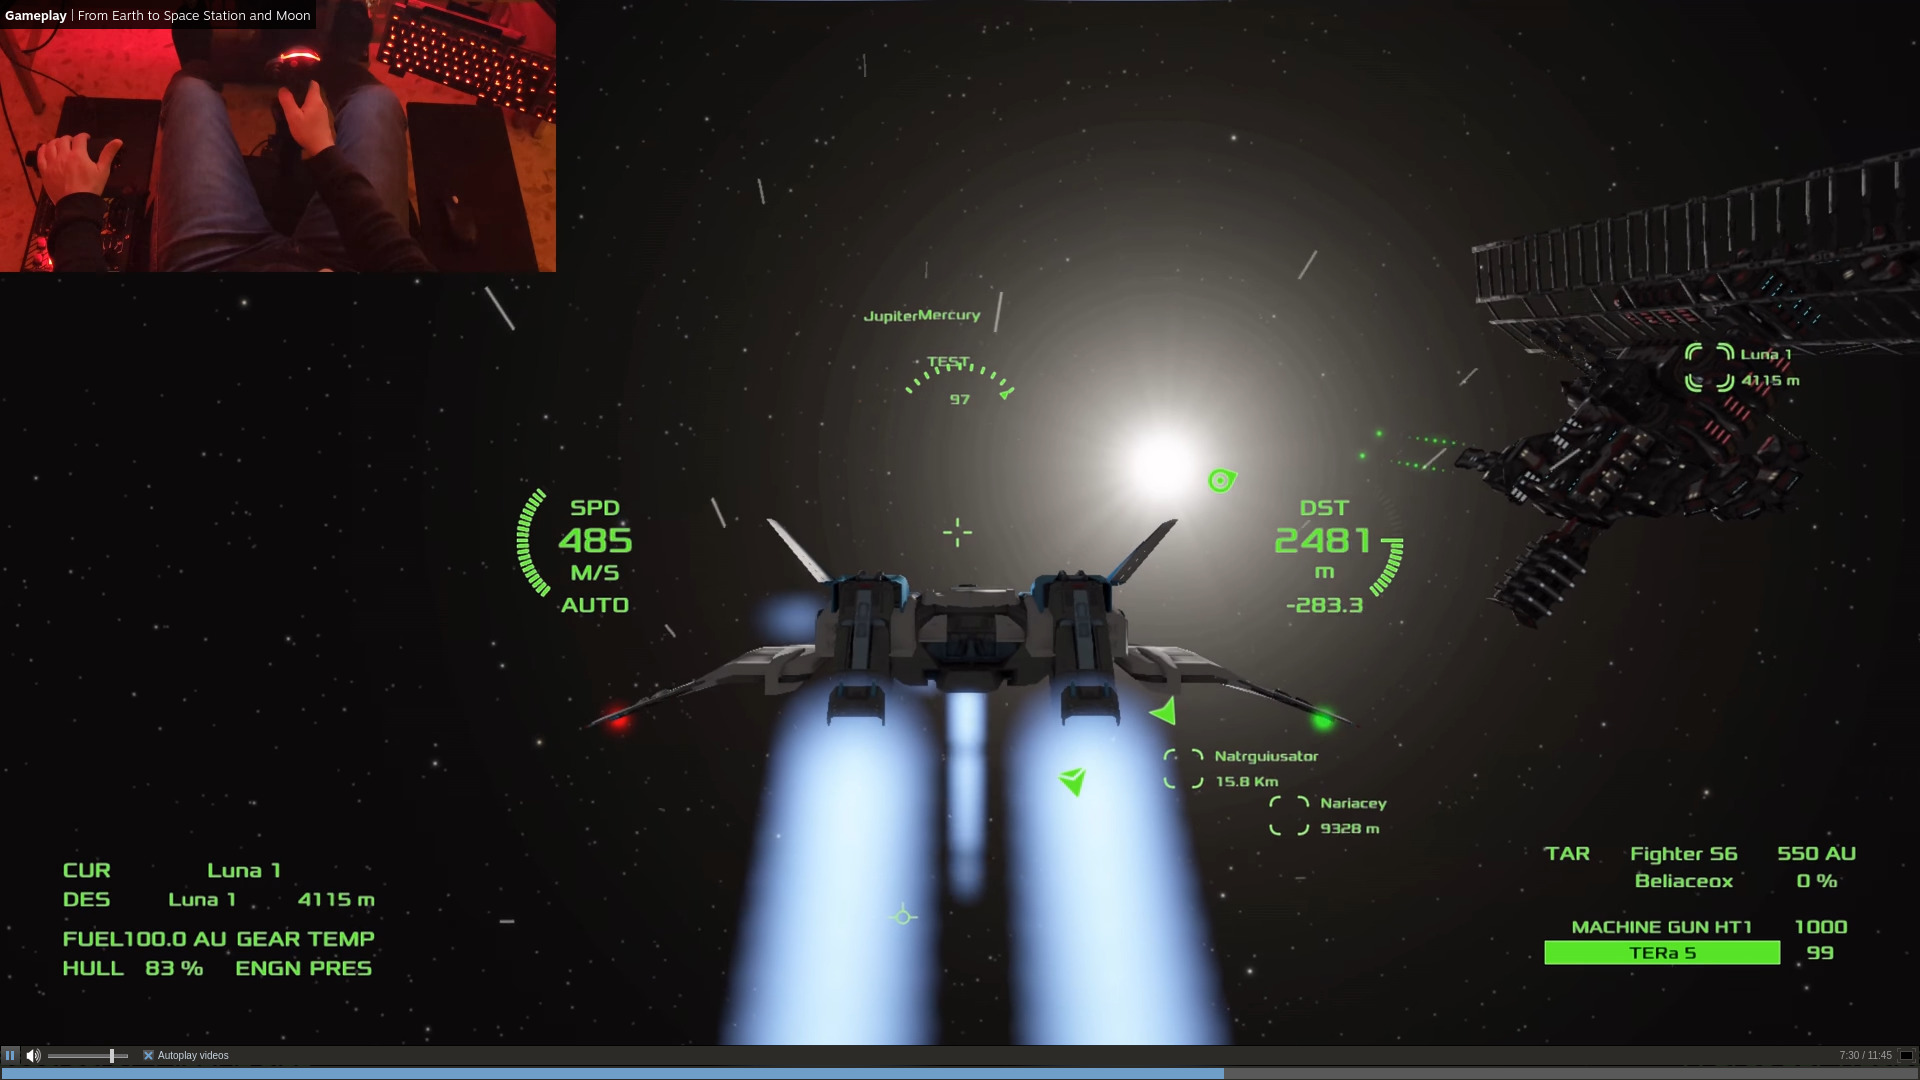
\includegraphics[width=\textwidth]{univoyager}\\
      \href{https://www.univoyager.com/}{Univoyager}
    \end{center}
  \end{minipage}
\end{frame}

\begin{frame}
  \frametitle{Space Flight Simulator Examples}
  \begin{minipage}[t]{0.49\textwidth}
    \begin{center}
      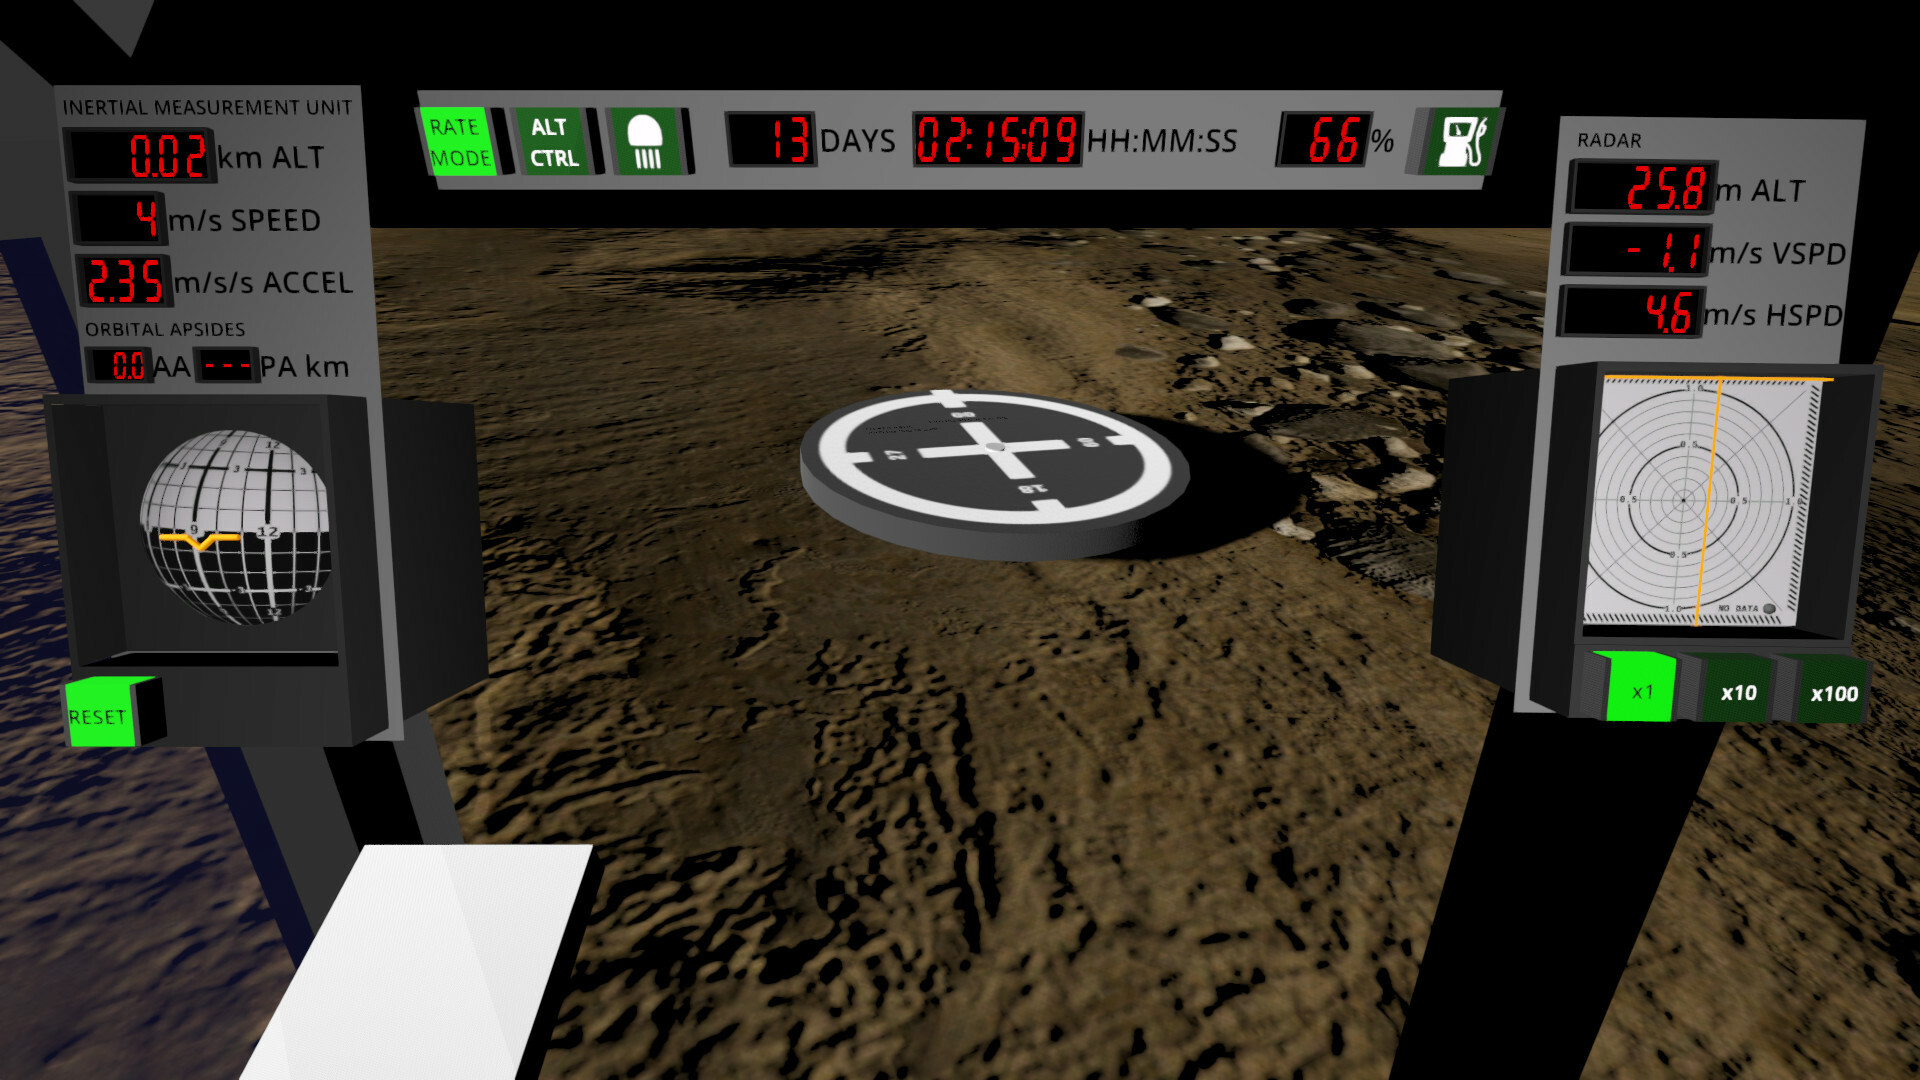
\includegraphics[width=\textwidth]{tungsten-moon}\\
      \href{https://tungstenmoon.com/}{Tungsten Moon}
    \end{center}
  \end{minipage}
  \begin{minipage}[t]{0.49\textwidth}
    \begin{center}
      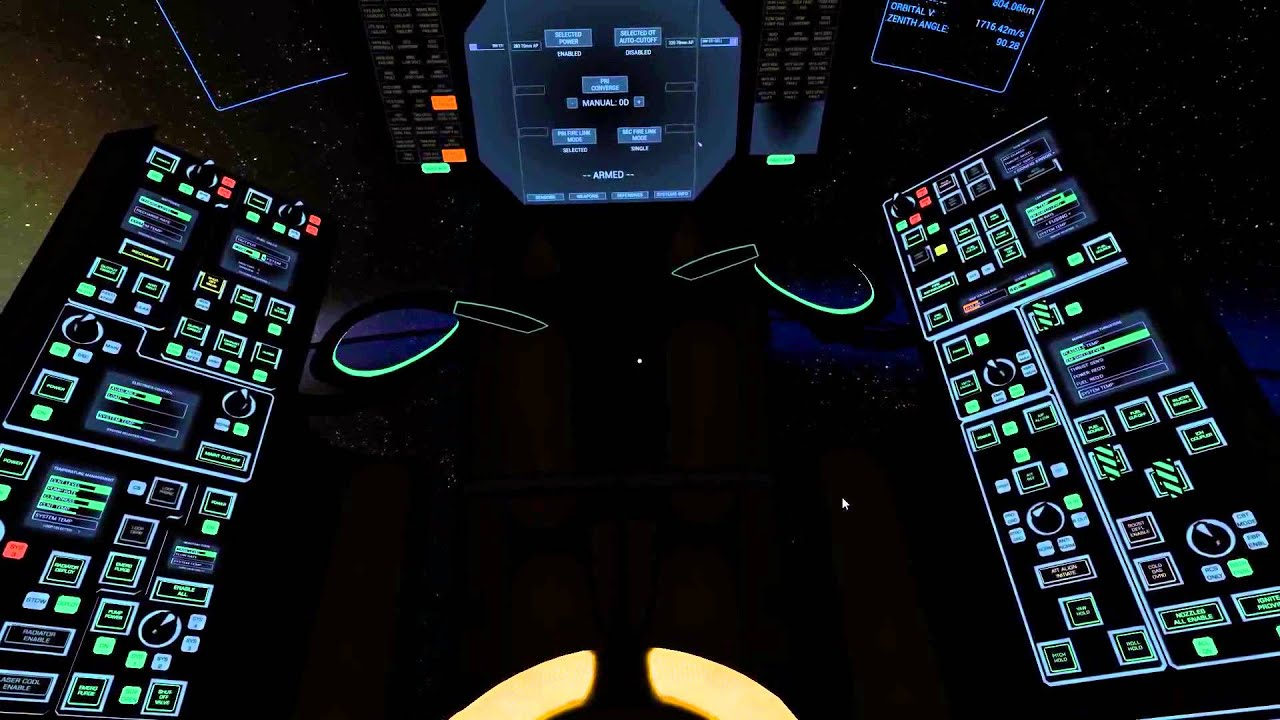
\includegraphics[width=\textwidth]{rogue-system}\\
      \href{https://imagespaceinc.com/rogsys/}{Rogue System}
    \end{center}
  \end{minipage}
\end{frame}

\begin{frame}
  \pdfbookmark[1]{questions}{questions}
  \begin{center}
    \begin{huge}
      Thanks for listening!
    \end{huge}
  \end{center}
\end{frame}

\end{document}
